\documentclass[../main.tex]{subfiles}
% !TEX root= ../main.tex
 
\begin{document}

\begin{center}
    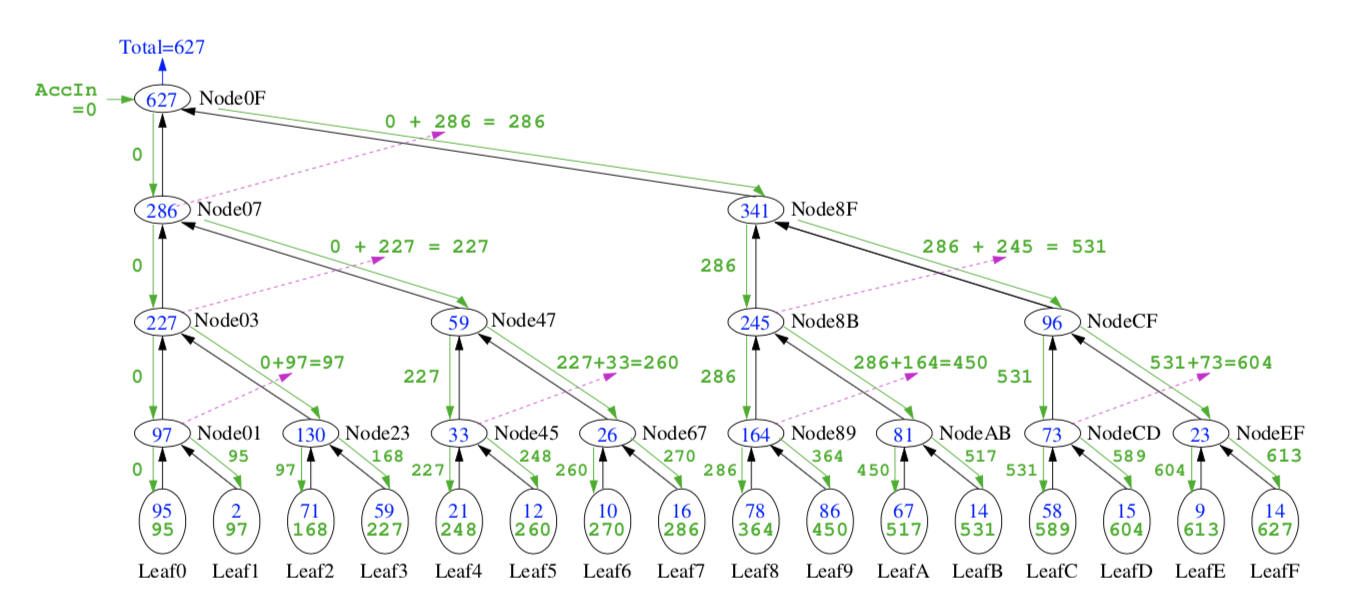
\includegraphics[scale=0.5]{images/scan.png}
\end{center}

\begin{itemize}
    \item Scan in two passes    
	\item Upward Pass: Reduce
	      \begin{itemize}
		      \item Each node receives values from left and right subtrees.
		      \item The node combine these values, and send the results to the parent.
		      \item The combine at the root produces the total for all nodes.
	      \end{itemize}
	\item Downward Pass:
	      \begin{itemize}
		      \item Each node has the values from its left and right children.
		      \item When a node receives a value from its parent:
		            \begin{itemize}
			            \item it sends the parent's value to its left subtree.
			            \item it combine the parent's value with the value from the left subtree and sends this to the right subtree.
		            \end{itemize}
		      \item When a leaf receives a value from its parent
		            \begin{itemize}
			            \item It combine this value with its own value and records that as its value as its result
		            \end{itemize}
	      \end{itemize}
\end{itemize}

\begin{lstlisting}[language=erlang]
    sum_scan(W, SrcKey, DstKey) ->
    wtree:scan(W,
        fun (ProcState) ->
            lists:sum(workers:get(ProcState, SrcKey)
        end,
        % Leaf1
        fun (ProcState, AccIn) -> % Leaf2
            MyList = workers:get(ProcState, SrcKey),
            {Result, _Total} = lists:mapfoldl(fun (E, Acc) -> V = E + Acc, {V, V} end, AccIn, MyList),
            workers:put(ProcState, DstKey, Result)
        end,
        fun (Left, Right) -> Left + Right end,
        % Combine
        0). % Acc0
\end{lstlisting}

\end{document}
